%% bare_conf_compsoc.tex
%% V1.4b
%% 2015/08/26
%% by Michael Shell
%% See:
%% http://www.michaelshell.org/
%% for current contact information.
%%
%% This is a skeleton file demonstrating the use of IEEEtran.cls
%% (requires IEEEtran.cls version 1.8b or later) with an IEEE Computer
%% Society conference paper.
%%
%% Support sites:
%% http://www.michaelshell.org/tex/ieeetran/
%% http://www.ctan.org/pkg/ieeetran
%% and
%% http://www.ieee.org/

%%*************************************************************************
%% Legal Notice:
%% This code is offered as-is without any warranty either expressed or
%% implied; without even the implied warranty of MERCHANTABILITY or
%% FITNESS FOR A PARTICULAR PURPOSE! 
%% User assumes all risk.
%% In no event shall the IEEE or any contributor to this code be liable for
%% any damages or losses, including, but not limited to, incidental,
%% consequential, or any other damages, resulting from the use or misuse
%% of any information contained here.
%%
%% All comments are the opinions of their respective authors and are not
%% necessarily endorsed by the IEEE.
%%
%% This work is distributed under the LaTeX Project Public License (LPPL)
%% ( http://www.latex-project.org/ ) version 1.3, and may be freely used,
%% distributed and modified. A copy of the LPPL, version 1.3, is included
%% in the base LaTeX documentation of all distributions of LaTeX released
%% 2003/12/01 or later.
%% Retain all contribution notices and credits.
%% ** Modified files should be clearly indicated as such, including  **
%% ** renaming them and changing author support contact information. **
%%*************************************************************************


% *** Authors should verify (and, if needed, correct) their LaTeX system  ***
% *** with the testflow diagnostic prior to trusting their LaTeX platform ***
% *** with production work. The IEEE's font choices and paper sizes can   ***
% *** trigger bugs that do not appear when using other class files.       ***                          ***
% The testflow support page is at:
% http://www.michaelshell.org/tex/testflow/



\documentclass[conference]{IEEEtran}
%\documentclass{IEEEtran}
% Some/most Computer Society conferences require the compsoc mode option,
% but others may want the standard conference format.
%
% If IEEEtran.cls has not been installed into the LaTeX system files,
% manually specify the path to it like:
% \documentclass[conference,compsoc]{../sty/IEEEtran}


%%%%%%%%%%%%%%%%%%%%%%%%%%%%%%%%%%%%%%%%%%%%%%%%%%%%%%%%%%
% Inline comments. Pick initials and color of your choice. \ysnote{} refers to Yogesh's note. 
%
\usepackage[usenames,dvipsnames,svgnames,x11names]{xcolor}
\newcommand{\ysnote}[1]{ {\textcolor{magenta} { ***Yogesh: #1 }}} % needs a response
\newcommand{\drnote}[1]{ {\textcolor{orange} { ***Dreamer: #1 }}}
\newcommand{\Note}[1]{\textcolor{red}{#1}} % verify if this is correct
\newcommand{\ysnoted}[1]{ {\textcolor{green} { ***TODO Later: #1 }}} % postpone addressing of comment

%%%%%%%%%%%%%%%%%%%%%%%%%%%%%%%%%%%%%%%%%%%%%%%%%%%%%%%%%%
% Additional fonts
\usepackage[T1]{fontenc} %% https://tex.stackexchange.com/questions/664/why-should-i-use-usepackaget1fontenc
\usepackage{lmodern} %% https://tex.stackexchange.com/questions/2369/why-do-the-less-than-symbol-and-the-greater-than-symbol-appear-wrong-as
\usepackage[normalem]{ulem} % required for strikeout font
% Default Computer Modern font (no bold implemented)
%\renewcommand{\ttdefault}{cmtt}
% Hence, Using Courier font
\renewcommand{\ttdefault}{pcr}


%%%%%%%%%%%%%%%%%%%%%%%%%%%%%%%%%%%%%%%%%%%%%%%%%%%%%%%%%%
% Change tracking for article revisions. Added, Deleted, Replaced, or Modified content.
%
\newcommand{\modc}[1]{{\textcolor{blue}{#1}}}
\newcommand{\addc}[1]{{\textcolor{teal}{#1}}}
\newcommand{\delc}[1]{ {\textcolor{gray} {\sout{#1}} }}
%\newcommand{\delc}[1]{} % uncomment this (and comment above line) to ignore showing deletion
\newcommand{\repc}[2]{ {\textcolor{gray} {\sout{#1}} }{\textcolor{teal} {#2}}}
%\newcommand{\repc}[2]{{\textcolor{teal}{#2}}} % uncomment this (and comment above line) to ignore showing deletion
%
%---------------------------------------------------------


%%%%%%%%%%%%%%%%%%%%%%%%%%%%%%%%%%%%%%%%%%%%%%%%%%%%%%%%%%
% *** MISC UTILITY PACKAGES ***
%
%\usepackage{ifpdf}
% Heiko Oberdiek's ifpdf.sty is very useful if you need conditional
% compilation based on whether the output is pdf or dvi.
% usage:
% \ifpdf
%   % pdf code
% \else
%   % dvi code
% \fi
% The latest version of ifpdf.sty can be obtained from:
% http://www.ctan.org/pkg/ifpdf
% Also, note that IEEEtran.cls V1.7 and later provides a builtin
% \ifCLASSINFOpdf conditional that works the same way.
% When switching from latex to pdflatex and vice-versa, the compiler may
% have to be run twice to clear warning/error messages.


%%%%%%%%%%%%%%%%%%%%%%%%%%%%%%%%%%%%%%%%%%%%%%%%%%%%%%%%%%
% *** CITATION PACKAGES ***
%
\usepackage[nocompress]{cite}
% cite.sty was written by Donald Arseneau
% V1.6 and later of IEEEtran pre-defines the format of the cite.sty package
% \cite{} output to follow that of the IEEE. Loading the cite package will
% result in citation numbers being automatically sorted and properly
% "compressed/ranged". e.g., [1], [9], [2], [7], [5], [6] without using
% cite.sty will become [1], [2], [5]--[7], [9] using cite.sty. cite.sty's
% \cite will automatically add leading space, if needed. Use cite.sty's
% noadjust option (cite.sty V3.8 and later) if you want to turn this off
% such as if a citation ever needs to be enclosed in parenthesis.
% cite.sty is already installed on most LaTeX systems. Be sure and use
% version 5.0 (2009-03-20) and later if using hyperref.sty.
% The latest version can be obtained at:
% http://www.ctan.org/pkg/cite
% The documentation is contained in the cite.sty file itself.
%
% Note that some packages require special options to format as the Computer
% Society requires. In particular, Computer Society  papers do not use
% compressed citation ranges as is done in typical IEEE papers
% (e.g., [1]-[4]). Instead, they list every citation separately in order
% (e.g., [1], [2], [3], [4]). To get the latter we need to load the cite
% package with the nocompress option which is supported by cite.sty v4.0
% and later.


%%%%%%%%%%%%%%%%%%%%%%%%%%%%%%%%%%%%%%%%%%%%%%%%%%%%%%%%%%
% When using XML fragments, using pretty-print is helpful.
%
\usepackage{listings}
% \usepackage{color}
% \definecolor{gray}{rgb}{0.4,0.4,0.4}
% \definecolor{darkblue}{rgb}{0.0,0.0,0.6}
%\definecolor{maroon}{rgb}{0.5,0,0}
% \definecolor{cyan}{rgb}{0.0,0.6,0.6}

\lstset{
  basicstyle=\ttfamily,
  columns=fullflexible,
  showstringspaces=false,
  commentstyle=\color{gray}\upshape,
  escapeinside={||},
  mathescape=true
}

\lstdefinelanguage{XML}
{
basicstyle=\ttfamily\footnotesize,
  morestring=[b]",
  moredelim=[s][\bfseries\color{Maroon}]{<}{\ },
  moredelim=[s][\bfseries\color{Maroon}]{</}{>},
  moredelim=[l][\bfseries\color{Maroon}]{/>},
  moredelim=[l][\bfseries\color{Maroon}]{>},
  morecomment=[s]{<?}{?>},
  morecomment=[s]{<!--}{-->},
  commentstyle=\color{gray},
  stringstyle=\color{blue},
  identifierstyle=\color{red}
%  morekeywords={type,id,value,impl}% list your attributes here
}
%
%---------------------------------------------------------


%%%%%%%%%%%%%%%%%%%%%%%%%%%%%%%%%%%%%%%%%%%%%%%%%%%%%%%%%%
% Better control over verbatim text
\usepackage{moreverb}

%%%%%%%%%%%%%%%%%%%%%%%%%%%%%%%%%%%%%%%%%%%%%%%%%%%%%%%%%%
% for syntax/grammar
\usepackage[nounderscore]{syntax}

%%%%%%%%%%%%%%%%%%%%%%%%%%%%%%%%%%%%%%%%%%%%%%%%%%%%%%%%%%
\usepackage[pdftex]{graphicx}
% declare the path(s) where your graphic files are
\graphicspath{{./figures/}}
% and their extensions so you won't have to specify these with
% every instance of \includegraphics
\DeclareGraphicsExtensions{.pdf}
% graphicx was written by David Carlisle and Sebastian Rahtz. It is
% required if you want graphics, photos, etc. graphicx.sty is already
% installed on most LaTeX systems. The latest version and documentation
% can be obtained at: 
% http://www.ctan.org/pkg/graphicx
% Another good source of documentation is "Using Imported Graphics in
% LaTeX2e" by Keith Reckdahl which can be found at:
% http://www.ctan.org/pkg/epslatex
%
% latex, and pdflatex in dvi mode, support graphics in encapsulated
% postscript (.eps) format. pdflatex in pdf mode supports graphics
% in .pdf, .jpeg, .png and .mps (metapost) formats. Users should ensure
% that all non-photo figures use a vector format (.eps, .pdf, .mps) and
% not a bitmapped formats (.jpeg, .png). The IEEE frowns on bitmapped formats
% which can result in "jaggedy"/blurry rendering of lines and letters as
% well as large increases in file sizes.
%
% You can find documentation about the pdfTeX application at:
% http://www.tug.org/applications/pdftex

% Definitions for placeholder figures
\newcommand{\dummyfigX}{\fbox{\parbox[h][1.75in][t]{0.95\textwidth}{\emph{Placeholder}}}} % full page width (figure*)
\newcommand{\dummyfigXX}{\fbox{\parbox[h][1.75in][t]{0.95\columnwidth}{\emph{Placeholder}}}} % 1 column width (in 2 column format)
\newcommand{\dummyfigXXX}{\fbox{\parbox[h][1.75in][t]{0.30\textwidth}{\emph{Placeholder}}}} % 1/3 full page width (figure*)
\newcommand{\dummyfigXXXX}{\fbox{\parbox[h][1.75in][t]{0.23\textwidth}{\emph{Placeholder}}}} % 1/4 full page width (figure*)


%%%%%%%%%%%%%%%%%%%%%%%%%%%%%%%%%%%%%%%%%%%%%%%%%%%%
% *** MATH PACKAGES ***
%
\usepackage[cmex10]{amsmath}
\usepackage{amssymb}
\usepackage{mathtools}
\usepackage{amsthm}
\usepackage{amsfonts}
\newtheorem{cons}{Constraint}
%
% A popular package from the American Mathematical Society that provides
% many useful and powerful commands for dealing with mathematics.
%
% Note that the amsmath package sets \interdisplaylinepenalty to 10000
% thus preventing page breaks from occurring within multiline equations. Use:
%\interdisplaylinepenalty=2500
% after loading amsmath to restore such page breaks as IEEEtran.cls normally
% does. amsmath.sty is already installed on most LaTeX systems. The latest
% version and documentation can be obtained at:
% http://www.ctan.org/pkg/amsmath



%%%%%%%%%%%%%%%%%%%%%%%%%%%%%%%%%%%%%%%%%%%%%%%%%%%%
% *** SUBFIGURE PACKAGES ***
\usepackage{subfig} %[caption=false,font=footnotesize,labelfont=sf,textfont=sf]
%
% subfig.sty, written by Steven Douglas Cochran, is the modern replacement
% for subfigure.sty, the latter of which is no longer maintained and is
% incompatible with some LaTeX packages including fixltx2e. However,
% subfig.sty requires and automatically loads Axel Sommerfeldt's caption.sty
% which will override IEEEtran.cls' handling of captions and this will result
% in non-IEEE style figure/table captions. To prevent this problem, be sure
% and invoke subfig.sty's "caption=false" package option (available since
% subfig.sty version 1.3, 2005/06/28) as this is will preserve IEEEtran.cls
% handling of captions.
% Note that the Computer Society format requires a sans serif font rather
% than the serif font used in traditional IEEE formatting and thus the need
% to invoke different subfig.sty package options depending on whether
% compsoc mode has been enabled.
%
% The latest version and documentation of subfig.sty can be obtained at:
% http://www.ctan.org/pkg/subfig




% *** SPECIALIZED LIST PACKAGES ***
%
\usepackage{algorithmicx}
\usepackage{algpseudocode}
\usepackage[ruled]{algorithm}
\definecolor{light-gray}{gray}{0.75}
\algrenewcommand{\algorithmiccomment}[1]{\hskip3em{{\footnotesize \textcolor{light-gray}{$\blacktriangleright$}}} #1}
%
% This package provides an algorithmic environment fo describing algorithms.
% You can use the algorithmic environment in-text or within a figure
% environment to provide for a floating algorithm. 


%%%%%%%%%%%%%%%%%%%%%%%%%%%%%%%%%%%%%%%%%%%%%%%%%%%%%%%%%%
% Table relates packages
\usepackage{multirow} % Multi-row tables
\usepackage{rotating} % sideways table
\usepackage{booktabs} % better lines
\usepackage{colortbl} % cell colors
\usepackage{tablefootnote} % add support for footnote in table

%%%%%%%%%%%%%%%%%%%%%%%%%%%%%%%%%%%%%%%%%%%%%%%%%%%%%%%%%%
% *** PDF, URL AND HYPERLINK PACKAGES ***
%
%\usepackage[colorlinks,bookmarksopen,bookmarksnumbered,citecolor=red,urlcolor=red]{hyperref}
\usepackage[pdftex,colorlinks=true,urlcolor=blue,citecolor=blue]{hyperref}


%%%%%%%%%%%%%%%%%%%%%%%%%%%%%%%%%%%%%%%%%%%%%%%%%%%%%%%%%%
% Avoids contiguous empty spaces
\usepackage{xspace}

%%%%%%%%%%%%%%%%%%%%%%%%%%%%%%%%%%%%%%%%%%%%%%%%%%%%%%%%%%
% IEEETrans class fix for enumitem. provide for legacy IED commands/lengths when possible
% http://comments.gmane.org/gmane.editors.lyx.general/68611
\let\labelindent\relax
\usepackage{enumitem}


%%%%%%%%%%%%%%%%%%%%%%%%%%%%%%%%%%%%%%%%%%%%%%%%%%%%%%%%%%
% correct bad hyphenation here
\hyphenation{compu-ta-tio-nal}

% define repetitive complex fragments here
\newcommand{\floe}{$\mathcal{F}{\ell}{o}{\varepsilon}$\xspace}
\newcommand{\prc}{\mathcal{P}}
\newcommand{\chn}{\mathcal{C}}


%%%%%%%%%%%%%%%%%%%%%%%%%%%%%%%%%%%%%%%%%%%%%%%%%%%%%%%%%%
% generate lorum ipsum placeholder text
%\usepackage[english]{babel}
\usepackage{blindtext}
\newcommand{\blindtextc}{\color{gray}\blindtext\color{black}}
\newcommand{\Blindtextc}{\color{gray}\Blindtext\color{black}}




\begin{document}

\title{Distributed Knowledge Graph Querying on \\ Edge, Fog and Cloud}


\author{\IEEEauthorblockN{Shriram R.}\\
\IEEEauthorblockA{Department of Computational and Data Sciences\\
Indian Institute of Science, Bangalore 560012 INDIA\\
Email: shriramr@iisc.ac.in}
}


\maketitle


\begin{abstract}
Knowledge graphs with millions of vertices and edges are currently being used to enable smart devices and knowledge discovery. IoT (Internet of Things) devices are becoming the consumer and producer of such large graphs. Existing graph querying and processing systems are designed to run on commodity hardware. However, IoT applications need lightweight graph processing systems that can scale across large number of devices and  handle concurrent queries with low latency. In this project, a lightweight distributed graph querying engine is proposed which can natively scale across edge, fog and cloud devices. It supports declarative query model for vertex, edge, reachability, shortest path and subgraph pattern mining queries. The engine has a novel caching, indexing and query partitioning mechanism which enables to scale efficiently with graph size and query workload. The engine is evaluated on a large scale virtual IoT testbed with massive real-world knowledge graphs. The results indicate that the engine can provide x\% lower latency on a diverse query workload and can handle y\% more queries concurrently compared to the baseline system.
\end{abstract}

\section{Problem Description}
The problem that is being solved in this project is the scaling of graph querying on edge, fog and cloud devices which can provide low-latency query response for many concurrent queries on massive knowledge graphs. \emph{Figure 1} shows a representation of typical edge-fog-cloud layout. There is a hierarchical structure where fogs can communicate with edges and cloud and the edges can directly communicate with only fog. Each edge is associated with a single fog depending on its spatial proximity or any other parameter. The bandwidth and latency of edge-fog, fog-fog and fog-cloud network links are significantly different from each other.

The edge, fog and cloud devices are heterogenous and have different compute and storage capabilities. In addition, the device failure rate varies across the layers with edge having the highest failure rate. In this project however, all the devices are considered to be 100\% reliable.

Existing graph processing/querying systems are designed for commodity hardware and cannot be efficiently deployed on low powered edge devices like smartphones, smart home appliances etc. These systems do not take into account the network hierarchy and device heterogeneity that exists on the current edge-fog-cloud layout. The proposed graph querying engine uses GoDB which is a distributed graph database as the backend and implements the novel features on top of the database.

\begin{figure}[!t]
	\centering
	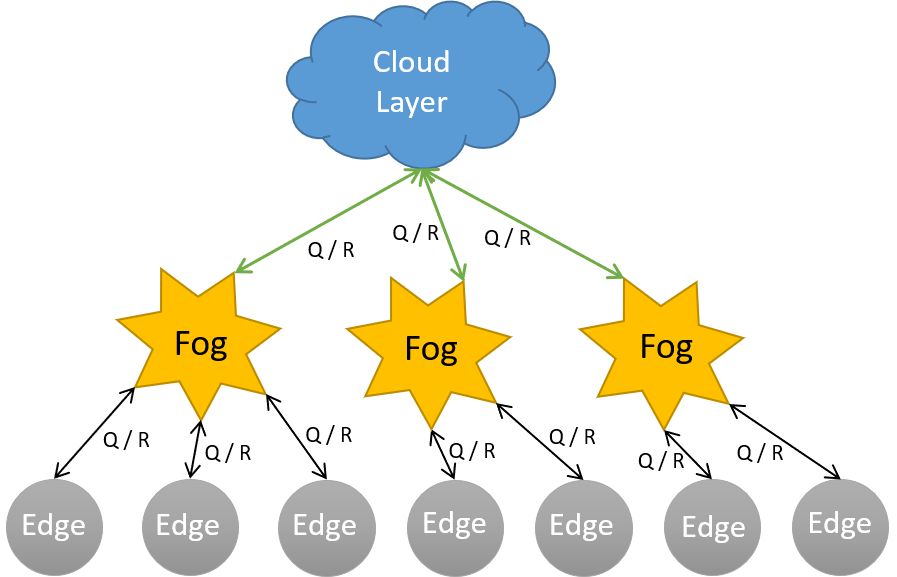
\includegraphics[width=0.75\columnwidth]{1.png}
	\caption{Edge-Fog-Cloud Layout}
	\label{fig:1}
\end{figure}
In this project, following are the key contributions:
\begin{itemize}%[noitemsep,topsep=0pt,parsep=0pt,partopsep=0pt]
	\item \textbf{Graph Partitioning:} A novel graph partitioning approach is used which partitions the graph based on the edge device. This means that the portion of knowledge graph which is frequently required by a query source is identified and moved closer to the edge device which performs the query automatically 
	\item \textbf{Query Partitioning:} A query planner which can efficiently partition the query and its predicates according to graph locality and placement thereby optimizing query cost is implemented
	\item \textbf{Query Caching:} A novel query caching system is devised which caches recent queries by edges and their corresponding results in the fog layer. It exploits the temporal and spatial locality of queries to provide low latency response. It also has a novel cache replacement policy and can quickly match an incoming query with cache. 
	\item \textbf{Graph Indexing} Index data structures from existing literature that can accelerate the processing of queries are built in a distributed fashion and are used for pruning the knowledge graph for processing. Different type of indexes are built for each query type and are maintained dynamically as per updates to the knowledge graph    
\end{itemize}

\section{Novelty/Scalability}
This problem is novel and has the following scalability challenges: The size of real-world knowledge graph data is massive with respect to the storage available in edges. For example, YAGO\cite{Suchanek:2007:YCS:1242572.1242667} which is a semantic knowledge base has about 10 million nodes and 120 million edges along with various properties. It has a total size of 170 GB (uncompressed).

Many of the graph mining problems and pattern matching (subgraph isomorphism) are NP complete which means that they cannot be feasibly computed in real time using just the edge devices. 

The knowledge graphs are relatively dynamic in nature with multiple updates throughout the graph happening in a short time interval. This poses a challenge in terms of building and updating indexes rapidly.

Graph partitioning is non-trivial due to the structure and heterogeneity of edge-fog-cloud. Many of the IoT applications require real-time answers whereas the existing distributed graph engines typically address batch processing queries with high latency.

An edge-fog-cloud system deployed on a city-wide network can have on the order of thousands of devices.  The query engine has to efficiently scale to this size and simultaneously provide acceptable level of performance.

Existing query engines are built on platforms or frameworks that are resource heavy. In order to run the proposed engine on the edge device, a significant optimization of the system in terms of resource requirements is necessary. 

\section{Related Work}

\emph{Pregel}\cite{Malewicz:2010:PSL:1807167.1807184}, \emph{Giraph}\cite{Ching:2015:OTE:2824032.2824077} and \emph{GraphX}\cite{Xin:2013:GRD:2484425.2484427} are designed as batch mode graph processing frameworks for commodity clusters which are not suitable for interactive queries.

\emph{Trinity}\cite{Shao:2013:TDG:2463676.2467799} is a distributed graph engine built as a in-memory key-value store. Though it is possible to perform interactive graph querying, the engine depends on high-speed network and requires large memory both of which are not feasible in edge-fog-cloud.

\emph{GC}\cite{enlighten130141} focusses on caching graph queries and results for graph isomorphism problems. It also provides novel cache replacement strategies for different workloads. However, it does not address other query types and is not designed for hierarchical device layout like in our case.

\emph{C-Tree}\cite{1617406} and \emph{Views}\cite{6816650} provide efficient indexing techniques for subgraph isomorphism queries. However, these indexes are not designed for distributed systems where the index has to be partitioned along with the graph data.

\emph{FERRARI}\cite{6544893} describes an efficient index for reachability and path queries. However, it is not straightforward to translate the design for our distributed setup.

\emph{GraphS}\cite{Qiu:2018:RCC:3229863.3275554} provides an efficient indexing technique to perform cycle detection in large distributed dynamic graphs with low latency. Our engine can adopt this technique for heterogenous device setup.  

\emph{GoDB}\cite{jamadagni:ccgrid:2016} is one of the closest work to the proposed engine. It is a distributed graph database which supports declarative queries on large property graphs. \emph{GoDB} is built on \emph{GoFFish}\cite{10.1007/978-3-319-09873-9_38} subgraph-centric batch processing platform thereby using its scalability.  

\emph{GoDB} supports vertex, edge, path and reachability queries. It also come with a novel cost model which uses execution heuristics to come with a optimum query plan that minimizes latency.

However, it is not designed to work on heterogenous device layout and is not capable of running on the edge devices. It comes with indexing mechanism for filtering vertices and edges based on properties but lack query type specific indexes which can dramatically reduce the query processing time.

\emph{GoDB} also do not have any caching mechanism and therefore cannot leverage on temporal and spatial locality of input queries. 

\emph{Quegel}\cite{Yan:2016:GQF:2904483.2904488} system provides a vertex centric programming model for processing graph on commodity clusters. It treats queries as first class citizens and uses a novel superstep-sharing execution model along with \emph{Hub} indexing technique to improve utilization of resources and performance.

However, it lacks a declarative query model and graph partitioning technique to support heterogenous devices and targets only commodity clusters.

It seems apparent that there are no graph querying system that solves the exact problem of graph querying in edge-fog-cloud. 

\section{Problem Definition and Approach}

The proposed graph engine consists of different modules spanning across the edge, fog and cloud layer. \emph{Figure 2} illustrates the high level architecture of the system. Additional details and functionalities present in each layer is given below,

\begin{figure*}[th]
	\centering%~%
	\subfloat[High Level Architecture]{
		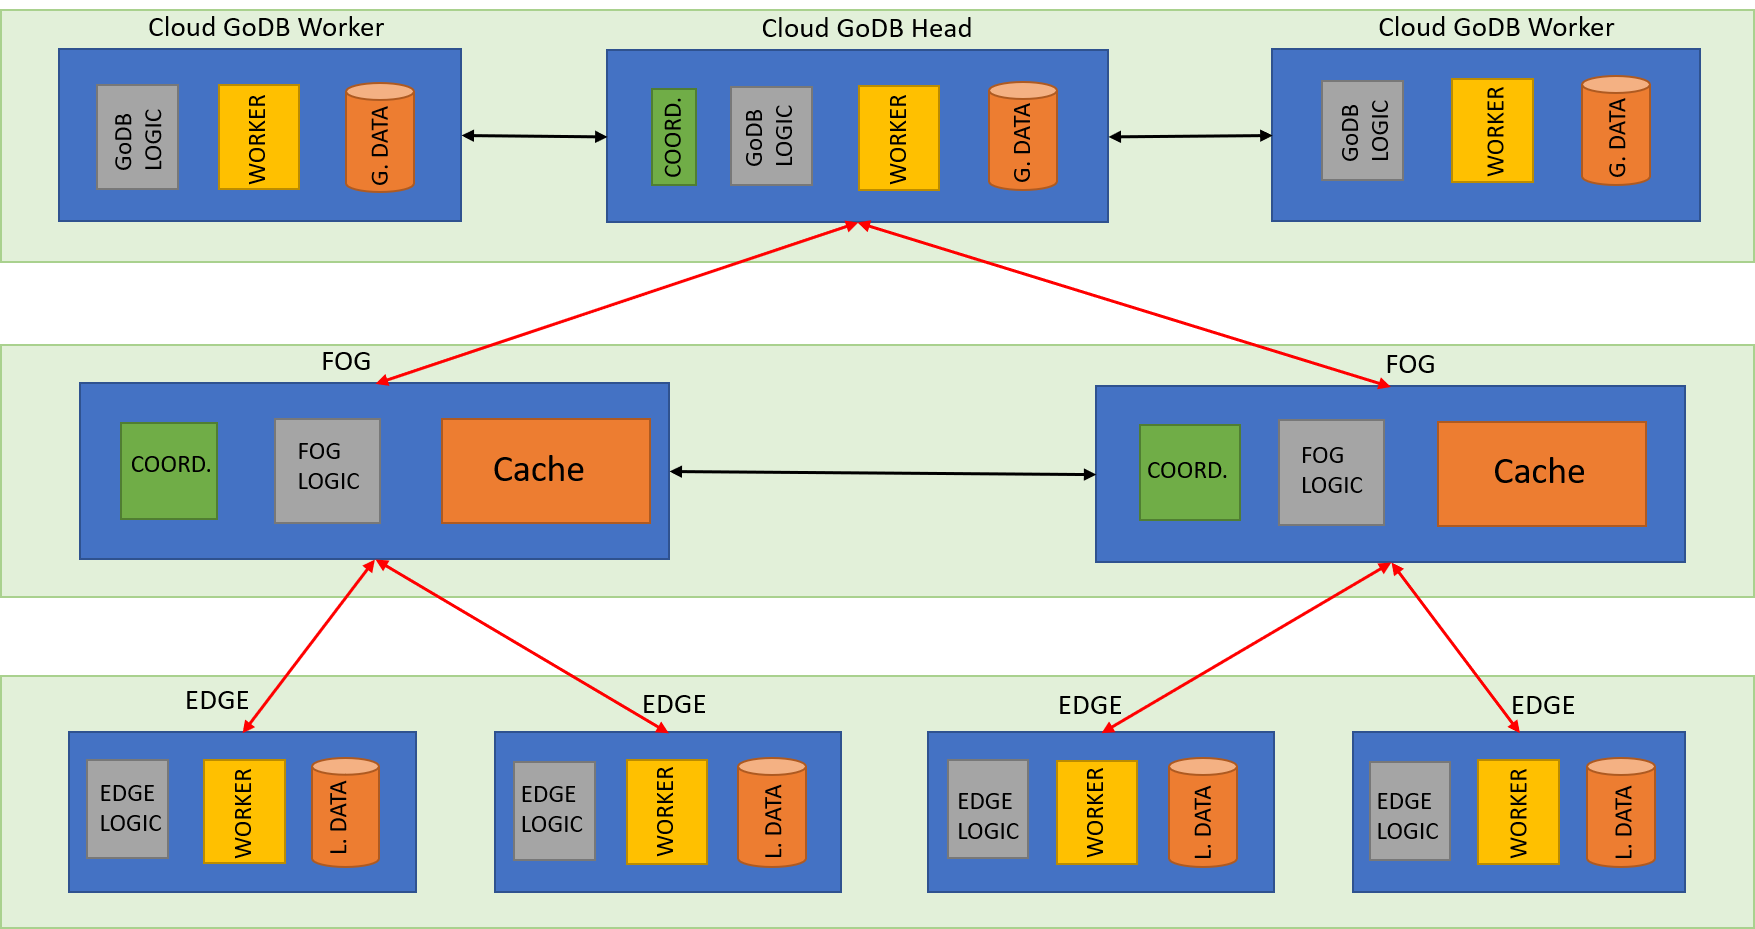
\includegraphics[height=0.23\textheight]{2.png}
		\label{fig:arch}
	}\qquad
	\subfloat[Logical Flow]{
		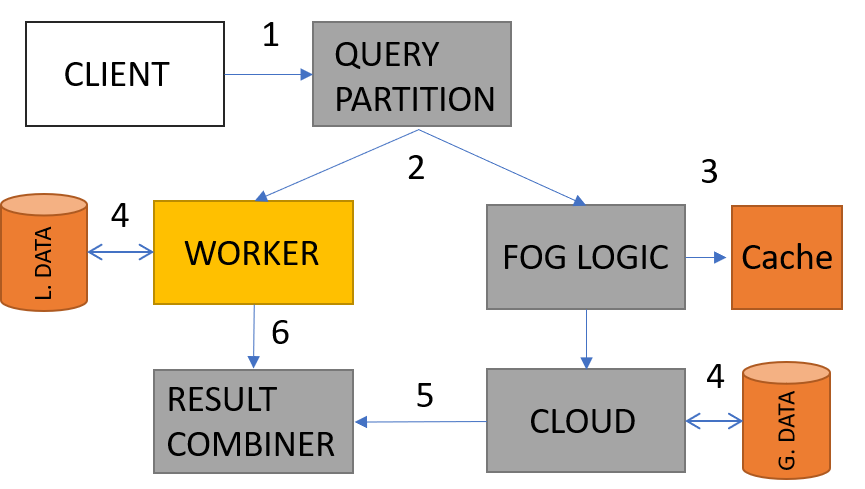
\includegraphics[height=0.15\textheight]{3.png}
		\label{fig:logic-flow}
	}\\
	\label{fig:problem-approach}
	\caption{Proposed Design}
	\vspace{-0.1in}
\end{figure*} 

\begin{itemize}%[noitemsep,topsep=0pt,parsep=0pt,partopsep=0pt]
	\item \textbf{Cloud Layer:} This layer consists of multiple nodes (VMs) that are interconnected. One of these nodes is a the Head or master node while the other nodes are the workers. GoDB database engine is deployed on top of these nodes and serve as the core graph querying engine. These nodes are commodity grade. The global knowledge graph is hosted in the GoFS data storage
	\item \textbf{Fog Layer: } Fog layer consists of three essential modules. The Cache module consists of statistics manager for maintaining the statistics, cache replacement logic and cache store for storing the queries and their corresponding results. The Fog logic module is responsible for sending the query to cloud, retrieve the results and pass them to edge. It also performs cache check for any incoming query from the edge. The coordination module is used to manage the edges which includes edge discovery and communicate with other fogs
	\item \textbf{Edge Layer: }	Edge layer consists of a local data store which stores the local knowledge graph. This partition of graph is assumed to queried most frequently by the corresponding edge. Each edge consists of a worker which performs graph processing locally. There is a edge logic module that includes the logic for query partitioning and result combiner 
\end{itemize}

\emph{Figure 2} shows the logical flow for a single query from query submission to obtaining the results. A detailed description of each step is given below,

\begin{enumerate}%[noitemsep,topsep=0pt,parsep=0pt,partopsep=0pt]
	\item The graph query in declarative language is submitted to the edge from a client. The client could very well be the edge itself. The proposed design should can be trivially extended to handling clients in fog and cloud. Only edge level clients are covered in this section
	\item The query partition logic essentially splits the input query into two. One part of the query is run on the edge using the local knowledge graph and the other part is sent to the fog layer. The objective of this partitioning is to run the query in parallel on both edge and cloud and merge the results
	\item The fog logic receives the global query from edge and checks the cache first for a hit. It will also send the query to neighbouring fogs to check for cache hit to allow for spatial locality. If there is a cache hit, the fog retrieves the query result or else it contacts the cloud layer to retrieve the result. 
	\item The edge worker receives the local query and start the processing for the given query type. The worker follows subgraph centric model similar to GoDB and the entire local knowledge graph is treated as a single subgraph for this purpose. The cloud head node receives the global query in parallel and computes the result using the worker nodes. 
	\item Once the result is computed in cloud, it is sent to result combiner in edge through the parent fog. Note that this is only a partial result for the original input query
	\item The local worker on the edge finishes its task and sends the result to the combiner. The combiner logic then merges the result from edge and cloud using a query type specific logic and sends the merge result to the client 
\end{enumerate}

The graph partitioning between edges and cloud happens by specifying a central vertex for each edge device. The central vertex along with its neighbours within a specified distance is captured and stored as the local knowledge graph.

For the purpose of this project, the knowledge graph is assumed to be static. For dynamic graphs, additional logic is required in edge, fog and cloud to update the indexes, cache and the graph data itself.

The implementation in edge and fog will be done in Python language as it is known to be lightweight in terms resource requirement. The communication between the devices is handled through gRPC framework. Cache data in Fog layer will be in-memory as the fog layer is known to be reliable and will be spilled to disk only if necessary.

Graph indexing is considered as good to have functionality with respect to the scope of this project. It will be potentially stored along with the graph data and additional modules will be added in edge layer to make use of the indexes.

Also, depending upon the feasibility of deploying GoDB on the cloud, it might be necessary to replace it with other distributed graph database. This should not affect any functionality in the edge and fog as long as the interface is made constant.

Major implementation effort is needed to complete the worker and edge logic modules as these will have different logic for each query type. Feasibility of porting some of the query planning and optimization logic from GoDB will be explored before the actual implementation.

Additional details regarding the query partition and result combining logic is omitted due to lack of space. It will be added in depth in the final project report.

\section{Proposed Experiments}

The experimental setup is as follows: Microsoft Azure cloud platform will be used to run the entire edge-fog-cloud setup. 5 D4 VMs will be used to run the cloud layer. These VMs will host the GoDB head and worker nodes. GoDB uses GoFFish v2.6 and Java v1.7. VIoLET\cite{DBLP:journals/corr/abs-1806-06032} will be used to virtually emulate the fog and edge layer. 3 Fogs of type Nvidia TX1 will be created and each fog will connect to 20 edges of type Pi3B+. The latency and bandwidth of edge-fog, fog-fog and fog-cloud will be set to 1ms-50mbps, 1ms-100mbps and 5ms-20mbps respectively. All the devices will be running on CentOS v7.

The YAGO dataset will be the primary knowledge graph data that will be used for the experiments. NELL\cite{Mitchell:2018:NL:3210350.3191513} could be used as a secondary dataset. The baseline system for comparison will be GoDB in cloud layer with edges and fogs running all the queries directly on the cloud. The graph is partitioned using METIS with one subgraph per core.

The size of the knowledge graph that be accommodated inside the edge device will be determined through the following experiment - 1 query of each type will be triggered on the edge for different sizes of local graph which is doubled in each iteration. The same set of query will also be triggered in cloud and the time taken in both the cases will be measured. This size should be the maximum size in which the local query time is less than the global query time for the same subgraph. This size will be used in all the below experiments as well.

\textbf{Microbenchmarks}
\begin{enumerate}%[noitemsep,topsep=0pt,parsep=0pt,partopsep=0pt]
	\item Query partitioning logic will incur some time to partition the query and generate a query plan. It is useful to measure this time for each query type. An experiment is performed with 100 different queries for each type being run on the edge and the time to partition is measured and plotted as a violin plot. The violin should ideally not have long tails.
	\item Graph indexing time and memory has to be measured for different query types as a function of graph size. In this experiment, for each graph size, index construction time and index size is measured for each index type. The time taken and size should increase as per the time and space complexity of the index.
\end{enumerate}

The experiments will test the impact of query partitioning, query caching and graph indexing and the metric to measured is the query latency.  

\begin{enumerate}%[noitemsep,topsep=0pt,parsep=0pt,partopsep=0pt]
	\item \textbf{Query Partitioning:} 100 random queries of each type (Vertex, Edge, Reachability, Shortest path and Subgraph isomorphism) will be triggered in total with the queries uniformly and randomly distributed across all the edges. The time taken to complete the query in the local knowledge graph, the global knowledge graph and query completion time is measured. When compared with baseline, the query completion time should be less in the new system and the local querying time should be far less than the global time since the size of local graph will be smaller compared to the global graph. This showcases the effectiveness of Query Partitioning on the performance.
    \item \textbf{Query Caching:} There will be two baselines for comparison. One is the cloud only baseline and the other is the edge-fog-cloud setup with cache disabled. In this experiment, each edge will have 20 different queries. These queries will be executed 5 times each in random order. This is to enable repetition of the same query from a given edge device. The time taken to complete the query in local and global graph and the total time will be measured. The cache hit/miss count will also be logged for each query execution. The cache enabled version should ideally outperform the other two baselines in terms of global execution time since the global query result will be cached in the fog.
    \item \textbf{Graph Indexing:} The baseline for graph indexing will be edge-fog-cloud setup with indexing disabled on the edge. This experiment consists of 100 random queries of each type similar to the Query Partitioning experiment. The time taken to complete the local query with index and without index is measured. The outcome should be that the time taken with index should be less than the without index baseline. The effectiveness of each index for each query type will be different since problems which are NP complete like subgraph isomorphism will offer more benefit in having the index than other simple problems like vertex or edge search.
\end{enumerate}


% trigger a \newpage just before the given reference
% number - used to balance the columns on the last page
% adjust value as needed - may need to be readjusted if
% the document is modified later
\IEEEtriggeratref{6}
% The "triggered" command can be changed if desired:
%\IEEEtriggercmd{\enlargethispage{-5in}}

% references section

% can use a bibliography generated by BibTeX as a .bbl file
% BibTeX documentation can be easily obtained at:
% http://mirror.ctan.org/biblio/bibtex/contrib/doc/
% The IEEEtran BibTeX style support page is at:
% http://www.michaelshell.org/tex/ieeetran/bibtex/
\bibliographystyle{IEEEtran}
% argument is your BibTeX string definitions and bibliography database(s)
\bibliography{paper}

% that's all folks
\end{document}

%%% Local Variables:
%%% mode: latex
%%% TeX-master: t
%%% End:
